\documentclass[12pt,a4paper]{article}
\usepackage[T2A]{fontenc}
\usepackage[utf8]{inputenc}
\usepackage[russian]{babel}

\usepackage{graphicx}
\graphicspath{{img/}}
\DeclareGraphicsExtensions{.png}

\usepackage{float}
\usepackage{hyperref}
\usepackage[
top=2cm]{geometry} % для изменения размеров полей документа
\usepackage{amsmath}
\usepackage{amsfonts}
\usepackage{amssymb}

\begin{document}

\begin{titlepage}
	\newpage
	
	\begin{center}
		Санкт-Петербургский государственный политехнический 
		университет Петра Великого \\
		\vspace{1cm}
		Кафедра компьютерных систем и программных технологий\\*
%		\hrulefill
	\end{center}
	
	\vspace{8em}
	
	\begin{center}
		 Отчёт по лабораторной работе №1
	\end{center}
	
	\vspace{2.5em}

	\vspace{6em}
	\flushleft{Выполнила студентка гр.33501/3:Ивашкевич О.А.}

	\flushleft{Преподаватель: Богач Н.В.}
	\vspace{\fill}
	
	\begin{center}
		Санкт-Петербург
		
		 2017
	\end{center}
	
\end{titlepage}

\newpage

\section{Сигналы телекоммуникационных систем}

\subsection{Цель работы}

Познакомиться со средствами генерации и визуализации простых сигналов.

\subsection{Постановка задачи}

В командном окне MATLAB и в среде Simulink промоделировать сигналы из Главы 3, сс. 150–170 (см. Справочные материалы).

\subsection{Справочные материалы}

А.Б. Сергиенко Цифровая обработка сигналов. Глава 1,
сс.18–25, Глава 3, сс. 150–170.

\subsection{Ход работы}

Необходимо провести генерацию сигналов в MATLAB, используя программный код, предложенный на страницах методического пособия.
Для генерации сигнала необходимо сначала создать вектор дискретных значений времени.
Рассчитаем обратную величину частоты дискретизации Fs, вычисленное значение будет использоваться для временного шага при моделировании частоты.

\begin{verbatim}
Fs = 8e3;     % частота дискретизации 8 кГц
t = 0:1/Fs:1; % одна секунда дискретных значений времени
t = t';       % преобразуем строку в столбец
\end{verbatim}

Ниже приведена функция для вычисления значения сигнала в любой момент времени.

\begin{verbatim}
A = 2;                        % амплитуда - два вольта
f0 = 1e3;                     % частота - 1 кГц
phii = pi/4;                  % начальная фаза 45
s1 = A * cos(2*pi*f0*t + pi); % гармонический сигнал
alpha = 1e3;                  % скорость затуханий
s2 = exp(-alpha*t).*s1;       % затухающая синусоида
\end{verbatim}

Для получения графиков, иллюстрирующих дискретный сигнал, используются нижеприведенные функции.

\begin{itemize}
  \item Рис.~\ref{fig:img1}, a -- график зависимости U(t), где U - сигнал t-время, построенный с помощью plot, при этом отсчеты соединяются линиями;
  \item Рис.~\ref{fig:img1}, b -- тот же график, но отображены только отсчеты;
  \item Рис.~\ref{fig:img1}, c -- функция stem изображает сигнал в виде "<стебельков">;
  \item Рис.~\ref{fig:img1}, d -- функция stairs выводит график в ступенчатом виде.
\end{itemize}
Ниже приведена последовательность команд, для приведенных выше случаев:
\begin{verbatim}
subplot(2, 2, 1); plot(s2(1:100));      % с линиями
subplot(2, 2, 2); plot(s2(1:100), '.'); % только точки
subplot(2, 2, 3); stem(s2(1:100));      % <<стебельки>>
subplot(2, 2, 4); stairs(s2(1:100));    % ступеньки
\end{verbatim}
\begin{figure}[!h]
  \centering
  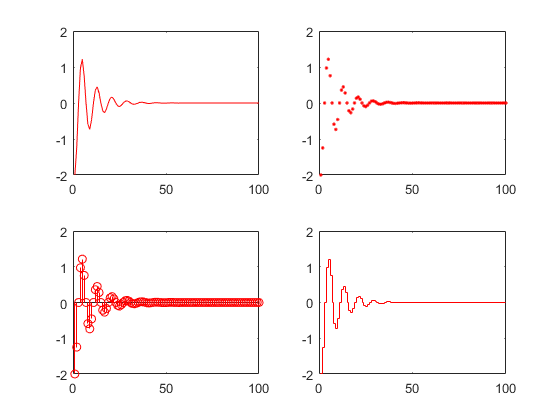
\includegraphics[width=\linewidth]{img1}
  \caption{Различные формы представления графиков дискретного сигнала.}
  \label{fig:img1}
\end{figure}

Ось абсцисс, на графиках Рис.~\ref{fig:img1}, проградуирована в номерах отсчетов. Чтобы показать на этой оси значения времени, можно подставить первым аргументом функций plot, stem или stairs вектор со значениями времени, например, так: \verb|plot(t(1:100), s2(1:100))| (Рис.~\ref{fig:img2}).
\begin{figure}[!h]
  \centering
  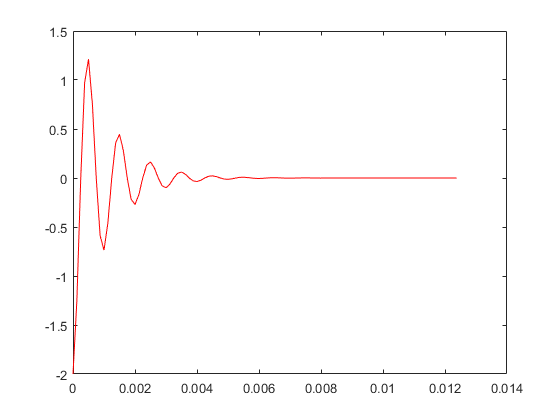
\includegraphics[width=\linewidth]{img2}
  \caption{График сигнала с корректно проградуированной временной осью.}
  \label{fig:img2}
\end{figure}

В MATLAB предоставляет возможность для генерации многоканального сигнала, каналы которого описываются одной и той же формулой, но с разными числовыми значениями параметров:
\begin{verbatim}
f = [600 800 1000 1200 1400]; % вектор частот (строка!)
s3 = cos(2*pi*t*f);           % пятиканальный сигнал
figure(3)
plot(t(1:100), s3(1:100, :));
\end{verbatim}
В результате \verb|s3| -- матрица, содержащая значения произведения времени и частоты. Итог вычислений показан на Рис.~\ref{fig:img3}:
\begin{figure}[!ht]
  \centering
  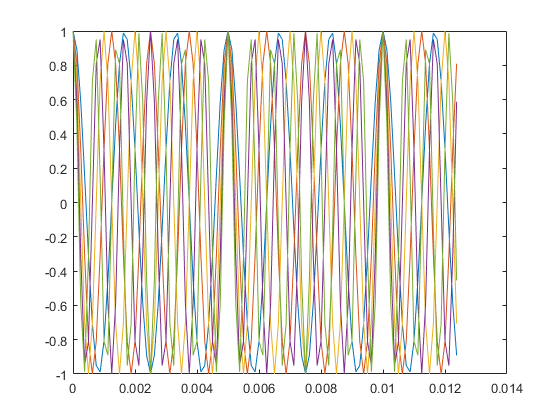
\includegraphics[width=\linewidth]{img3}
  \caption{Многоканальный сигнал.}
  \label{fig:img3}
\end{figure}

\subsubsection{Кусочные зависимости}
В MATLAB создание кусочных функций возможно провести несколькими способами.

Первый вариант -- использовать операцию сравнения, возвращающую значение 1, если условие выполняется, и 0 в противном случае. Этим можно воспользоваться для создания графиков, изображенных на Рис.~\ref{fig:img4}:
\begin{itemize}
  \item односторонний экспоненциальный импульс:
    \begin{verbatim}
    s4 = A*exp(-alpha*t).*(t >= 0);
    \end{verbatim}
  \item прямоугольный импульс, центрированный относительно начала отсчета времени:
    \begin{verbatim}
    Fs = 100;
    t = -1:1/Fs:1; % 2 секунды дискретных значений времени
    T = 0.5;
    s5 = A*(abs(t) <= T/2);
    \end{verbatim}
  \item несимметричный треугольный импульс:
    \begin{verbatim}
    s6 = A*t/T.*(t >= 0).*(t <= T);
    \end{verbatim}
\end{itemize}
\begin{figure}[!ht]
  \centering
  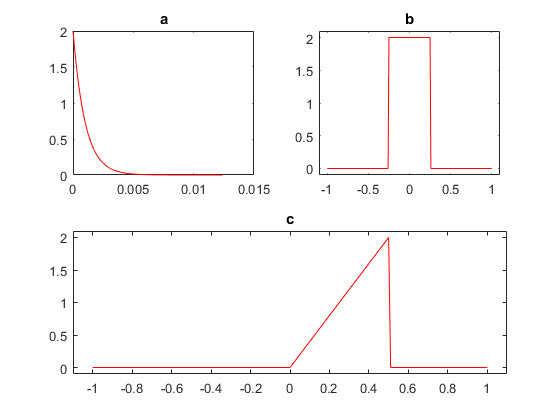
\includegraphics[width=\linewidth]{img4}
  \caption{Графики сигналов, полученные первым способом.}
  \label{fig:img4}
\end{figure}

Второй способ -- выполнять вычисления только для тех моментов времени, для которых это необходимо. Пример создания  трех кусочно-заданных сигналов:
\begin{itemize}
  \item a -- односторонний экспоненциальный импульс:
    \begin{verbatim}
    % заполняем вектор сигнала нулями
    s4 = zeros(size(t));
    % находим номера неотрицательных элементов вектора t*f
    inds = find(t >= 0);
    % рассчитываем сигнал только в нужных точках
    s4(inds) = A * exp(-alpha * t(inds));
    \end{verbatim}
      \item b -- прямоугольный импульс, центрированный относительно начала отсчета времени:
    \begin{verbatim}
    s5 = zeros(size(t));
    s5(find(abs(t) <= T/2)) = A;
    \end{verbatim}
      \item c -- несимметричный треугольный импульс:
    \begin{verbatim}
    s6 = zeros(size(t));
    inds = find((t>=0) & (t <= T));
    s6(inds) = A*t(inds)/T;
    \end{verbatim}
\end{itemize}
Результат визуализации не отличается от Рис.~\ref{fig:img4}.
% Кроме того, в пакете Signal Processing имеются следующие функции, генерирующие часто встречающиеся на практике непериодические сигналы:
% \begin{description}
% \item[rectpuls] -- прямоугольный импульс;
% \item[tripuls] -- треугольный импульс;
% \item[sinc] -- импульс вида $sin(\pi t)/(\pi t)$;
% \item[gauspuls] -- радиоимпульс с гауссовской огибающей;
% \item[pulstran] -- последовательность из конечного числа импульсов произвольной формы.
% \end{description}

% Рассмотрим их подробнее.

\subsubsection{Прямоугольный импульс}
Для формирования одиночного прямоугольного импульса с единичной амплитудой используется функция
\verb|y = rectpuls(t, width)|, где \verb|t| -- вектор значений времени, \verb|width| --  ширина импульса.
Возвращаемый результат \verb|y| -- вектор рассчитанных значений сигнала, определяемый формулой:
\begin{equation}
  y=
  \begin{cases}
    1, -\frac{width}{2} \leq t \leq \frac{width}{2}, \\
    0, t < -\frac{width}{2}, t \geq \frac{width}{2}.
  \end{cases}
\end{equation}

Пример создания прямоугольных импульсов с амплитудой 5 В и длительностью 20 мс каждый, расположенных справа и слева от начала отсчета времени. Результат показан на Рис.~\ref{fig:img_rectpuls}:
\begin{verbatim}
Fs = 1e3;              % частота дискретизации
t = -40e-3:1/Fs:40e-3; % дискретное время
T = 20e-3;             % длительность импульсов
A = 5                  % амплитуда
s = -A*rectpuls(t+T/2, T)+A*rectpuls(t-T/2,T);
plot(t,s);
ylim([-6 6]);
\end{verbatim}
\begin{figure}[!ht]
  \centering
  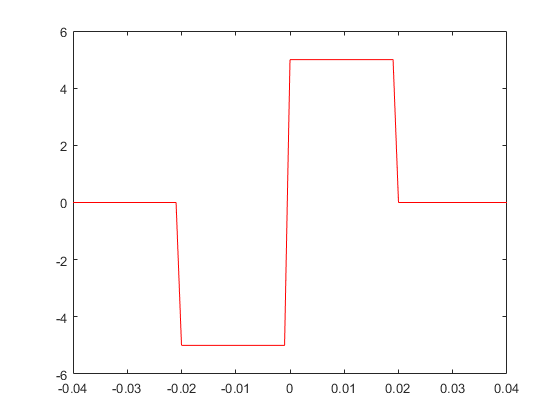
\includegraphics[width=\linewidth]{img_rectpuls}
  \caption{Сигнал, сформированный с помощью rectpuls.}
  \label{fig:img_rectpuls}
\end{figure}

\subsubsection{Треугольный импульс}
Для того, чтобы сформировать одиночный треугольный импульс с единичной амплитудой используется функция \verb|y = tripuls(t, width, skew)|, где \verb|t| -- вектор значений времени, \verb|width| --  ширина импульса, \verb|skew| -- коэффициент асимметрии импульса, определяющий положение его вершины. Пик импульса расположен при \verb|t=width*skew/2|. Параметр \verb|skew| должен лежать в диапазоне от -1 до 1.
Возвращаемый результат \verb|y| -- вектор рассчитанных значений сигнала, определяемый формулой:
\begin{equation}
  y=
  \begin{cases}
    \frac{2t+width}{width(skew+1)}, -\frac{width}{2} \leq t < \frac{width \cdot skew}{2}, \\
    \frac{2t-width}{width(skew-1)}, \frac{width \cdot skew}{2} \leq t < \frac{width}{2}, \\
    0, |t|>\frac{width}{2}.
  \end{cases}
\end{equation}

Ниже приведен пример формирования симметричного трапециевидного импульса с амплитудой 10 В и размерами верхнего и нижнего оснований 0 и 50 мс соответственно. Результат показан на Рис.~\ref{fig:img_tripuls}:
\begin{verbatim}
Fs = 1e3;
t = -50e-3:1/Fs:50e-3;
A = 10;
T1 = 20e-3;
T2 = 60e-3;
s = A*(T2*tripuls(t,T2)-T1*tripuls(t,T1))/(T2-T1);
plot(t,s);
\end{verbatim}
\begin{figure}[!ht]
  \centering
  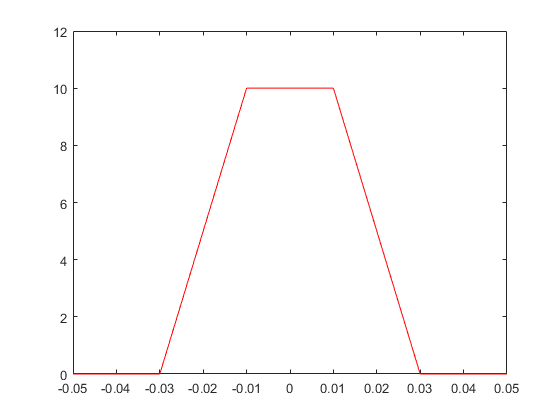
\includegraphics[width=\linewidth]{img_tripuls}
  \caption{Сигнал, сформированный с помощью tripuls.}
  \label{fig:img_tripuls}
\end{figure}

\subsubsection{Импульс с ограниченной полосой частот}
Для формирования сигнала, имеющего прямоугольный импульс, служит функция \verb|sinc(t)|, где \verb|t| -- то же, что и в предыдущих случаях.
Возвращаемый результат \verb|y| -- вектор рассчитанных значений сигнала, определяемый формулой:
\begin{equation}
  y=\frac{\sin(\pi x)}{\pi x}.
\end{equation}
Для примера построю график \verb|sinc| для линейного вектора (Рис.~\ref{fig:img_sinc}):
\begin{verbatim}
t = linspace(-5,5);
y = sinc(t);
plot(t,y);
xlabel('Time (sec)');
ylabel('Amplitude');
title('Sinc Function')
\end{verbatim}
\begin{figure}[!ht]
  \centering
  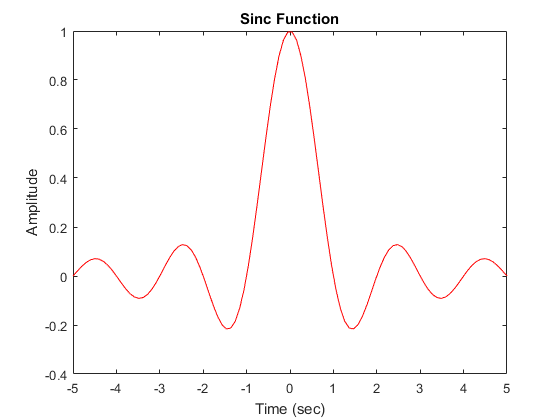
\includegraphics[width=\linewidth]{img_sinc}
  \caption{Сигнал, сформированный с помощью sinc.}
  \label{fig:img_sinc}
\end{figure}

\subsubsection{Гауссов радиоимпульс}
Формирование одиночного радиоимпульса с гауссовой огибающей и единичной амплитудой осуществляется при помощи специальной функции \verb|y = gauspuls(t, fc, bw, bwr)|, где \verb|t| -- вектор значений времени, \verb|fc| -- несущая частота в герцах, \verb|bw| -- относительная ширина спектра, \verb|bwr| -- уровень в децибелах, по которому производится измерение ширины спектра.
Возвращаемый результат \verb|y| -- вектор рассчитанных значений сигнала, определяемый формулой:
\begin{equation} \label{eq:gaus}
  y=\exp(-at^2)\cos(2\pi f_c t).
\end{equation}

Коэффициент \verb|a| используется для управляения длительностью импульса и шириной его спектра. Сигнал (\ref{eq:gaus}) имеет спектральную функцию, равную
\begin{equation}
  S(\omega) = \frac{1}{2} \sqrt{\frac{\pi}{a}} \left( \exp\left( -\frac{(\omega+2\pi f_c)^2}{4a} \right) + \exp\left( -\frac{(\omega-2\pi f_c)^2}{4a} \right) \right).
\end{equation}
Если $f_c \gg \sqrt{a}$, то можно пренебречь наложением "<хвостов"> сдвинутых копий спектра. Тогда параметр $a$ связан с относительной шириной спектра и уровнем (в дБ), по которому она определяется, следующим образом:
\begin{equation}
  a = -\frac{5(2\pi f_c \cdot bw)^2}{bwr \cdot \ln 10}
\end{equation}
Параметры $bwr$, $bw$ и $fc$ можно опустить, при этом используются их значения по умолчанию: $bwr=-6$ дБ, $bw=0.5$ и $fc=1000$ Гц.

При вызове функции \verb|gauspuls| используется от одного до трех выходных параметров: \verb|[y, yq, ye] = gauspuls()|. О значении второго и третьего выходного параметра можно узнать из справки MATLAB.

В качестве примера был сформирован гауссов радиоимпульс с несущей частотой 4 кГц и относительной шириной спектра 10\%, измеренной по уровню -20 дБ. Результат продемонстрирован на Рис.~\ref{fig:img_gaus}:
\begin{verbatim}
Fs = 16e3;             % частота дискретизации
t = -10e-3:1/Fs:10e-3; % дискретное время
Fc = 4e3;              % несущая частота
bw = 0.1;              % относительная ширина спектра
bwr = -20;             % уровень измерения ширины спектра
s = gauspuls(t, Fc, bw, bwr);
plot(t, s);            % график сигнала
ylim([-1.1 1.1]);
\end{verbatim}
\begin{figure}[!ht]
  \centering
  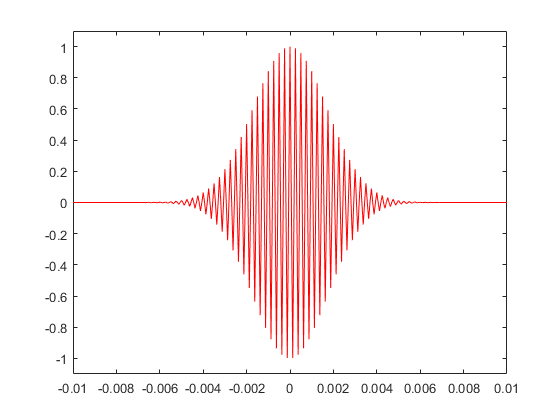
\includegraphics[width=\linewidth]{img_gaus}
  \caption{Сигнал, сформированный с помощью gauspuls.}
  \label{fig:img_gaus}
\end{figure}

Функция \verb|gauspuls| позволяет рассчитать \emph{время}, за которое огибающая гауссового импульса упадет до заданного уровня относительно максимума. При этом вместо вектора значений времени в качестве первого входного параметра используется строка '\verb|cutoff|': \verb|tc = gauspuls(| \verb|'cutoff', t, fc, bw, bwr, tpe)|, где \verb|tpe| -- уровень огибающей, момент достижения которого нужно определить. Возвращаемый результат \verb|tc| -- момент достиженигя оигбающей уровня \verb|tpe|.

В качестве примера рассчитывается время, за которое огибающая сформированного в предыдущем примере импульса уменьшается на 6 дБ (примерно в два раза):
\begin{verbatim}
>> gauspuls('cutoff', Fc, bw, bwr, -6)
ans =
    0.0020
\end{verbatim}

\subsubsection{Генерация последовательности импульсов}
Конечную последовательность импульсов (pulse train) одинаковой формы с произольно задаваемыми задержками и уровнями можно получить при помощи \verb|y=pulstran(t, d, 'func', p1, p2, ...)| -- если импульсы задаются именем генерирующей функции. Здесь \verb|t| -- вектор значений времени, \verb|d| -- вектор задержек, '\verb|func|' -- имя функции, генерирующей одиночный импульс. Оставшиеся параметры \verb|p1|, \verb|p2| и другие -- дополнительные, передающиеся функции \verb|func| при вызове.

В качестве примера используется последовательность из пяти симметричных треугольных импульсов, интервалы между которыми линейно увеличиваются, а амплитуды экспоненциально уменьшаются. Результат показан на Рис.~\ref{fig:img_pulstran}, a.
\begin{verbatim}
Fs = 1e3;                        % частота дискретизации
t = 0:1/Fs:0.5;                  % дискретное время
tau = 20e-3;                     % длительность импульса
d = [20 80 160 260 380]'*1e-3;   % задержки импульсов
d(:,2) = 0.8.^(0:4)';            % амплитуды импульсов
y = pulstran(t,d,'tripuls',tau);
plot(t, y)
\end{verbatim}
\begin{figure}[!ht]
  \centering
  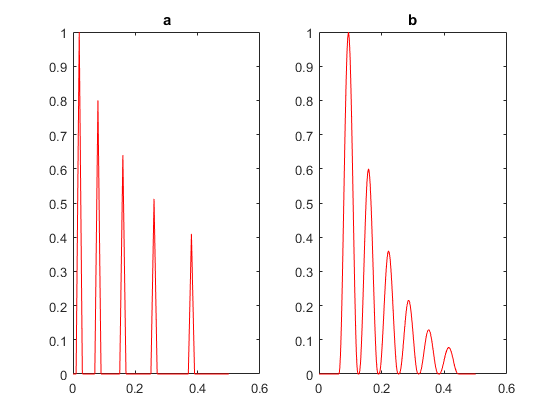
\includegraphics[width=\linewidth]{img_pulstran}
  \caption{Сигнал, сформированный с помощью pulstran.}
  \label{fig:img_pulstran}
\end{figure}

Если для генерации одиночного импульса нет готовой функции, то можно рассчитать вектор отсчетов импульса, а затем использовать второй вариант вызова функции: \verb|pulstran(t, d, p, fs, 'method')|.

Ниже приведен пример формирования последовательности из шести импульсовв, имеющих форму одного периода функции $\sin^2$. Результат показан на Рис.~\ref{fig:img_pulstran}, b.
\begin{verbatim}
Fs0 = 400;              % частота дискретизации
tau = 60e-3;            % длительность импульса
t0 = 0:1/Fs0:tau;       % дискретное время для импульса
s0 = sin(pi*t0/tau).^2; % вектор отсчетов импульса
% генерируем последовательность импульсов
Fs = 1e3;               % частота дискр. послед-сти
t = 0:1/Fs:0.5;         % дискретное время для посл-сти
d = (1:6)'*64e-3;       % задержки импульсов
d(:,2) = 0.6.^(0:5)';   % амплитуды импульсов
y = pulstran(t,d,s0,Fs0);
plot(t,y);
\end{verbatim}

\subsubsection{Последовательность прямоугольных импульсов}
Последовательность прямоугольных импульсов можно сформировать с помощью функции \verb|y = square(t)|, где \verb|t| -- вектор значений времени. Последовательность будет иметь период $2\pi$ и скважность 2. С помощью второго входного параметра '\verb|duty|' можно регулировать скважность.

Сформировать последовательность с периодом $T$ можно так: $y=square(2\pi*t/T)$.

Пример последовательности однополярных прямоугольных импульсов с амплитудой 3 В, частотой следования 50 Гц, длительностью 5 мс. Результат на Рис.~\ref{fig:img_square}.
\begin{verbatim}
Fs = 1e3;              % частота дискретизации
t = -10e-3:1/Fs:50e-3; % дискретное время
A = 3;                 % амплитуда
f0 = 50;               % частота следования импульсов
tau = 5e-3;            % длительность импульсов
s = (square(2*pi*t*f0, f0*tau*100)+1)*A/2;
plot(t,s)
ylim([0 5])
\end{verbatim}
\begin{figure}[!ht]
  \centering
  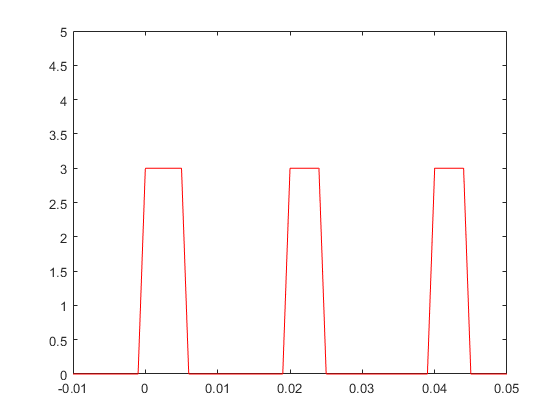
\includegraphics[width=\linewidth]{img_square}
  \caption{Последовательность прямоугольных импульсов, полученная с помощью функции square.}
  \label{fig:img_square}
\end{figure}

\subsubsection{Последовательность треугольных импульсов}
Формирование последовательности треугольных импульсов происходит с использованием функции \verb|y = sawtooth(t)|, где \verb|t| -- то же, что и в предыдущем случае. Период -- $2\pi$. C помощью второго параметра \verb|width| можно регулировать длительность "<обратного хода">. По умолчанию этот параметр равен единице.

Сформировать последовательность с периодом $T$ можно так: $y=sawtooth(2\pi*t/T)$.

В качестве примера построена  последовательность треугольных импульсов отрицательной полярности с амплитудой 5 в, периодом 50 мс и длительностью падающего участка 5 мс. Результат приведен на Рис.~\ref{fig:img_sawtooth}.
\begin{verbatim}
Fs = 1e3;               % частота дискретизации
t = -25e-3:1/Fs:125e-3; % дискретное время
A = 5;                  % амплитуда
T = 50e-3;              % период
t1 = 5e-3;              % длительность падающего участка
s = (sawtooth(2*pi*t/T, 1-t1/T)-1)*A/2;
plot(t,s)
\end{verbatim}
\begin{figure}[!ht]
  \centering
  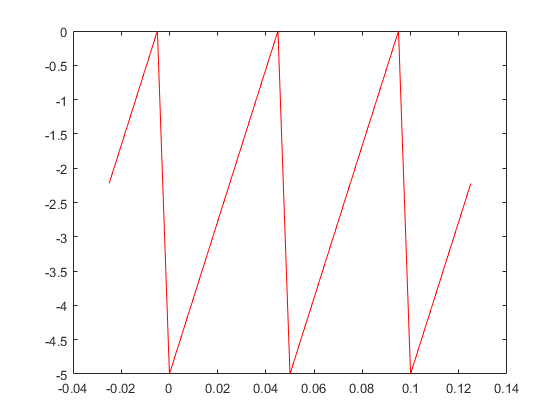
\includegraphics[width=\linewidth]{img_sawtooth}
  \caption{Последовательность прямоугольных импульсов, полученная с помощью функции sawtooth.}
  \label{fig:img_sawtooth}
\end{figure}

\subsubsection{Функция Дирихле}
Функция Дирихле описывается следующей формулой
\begin{equation} \label{eq:diric}
\mathrm{diric}_n(x)=\sum_{k=-\infty}^{\infty} \mathrm{sinc} \left( n \left(\frac{t}{2\pi}-k\right) \right),
\end{equation}
где $n$ -- целое положительное число.

Сформировать такую последовательность можно при помощи функции \verb|y=diric(x,n)|, где \verb|x| и \verb|n| соответствуют формуле (\ref{eq:diric}).

Для примера построил графики функции Дирихле при нечетном и четном значениях $n$ ($n=7$ и $n=8$, Рис.~\ref{fig:img_diric}).
\begin{verbatim}
x = 0:0.01:15;
subplot(2,1,1);
plot(x, diric(x, 7));
grid on;
title('n = 7');
subplot(2,1,2);
plot(x, diric(x, 8));
grid on;
title('n = 8');
\end{verbatim}
\begin{figure}[!ht]
  \centering
  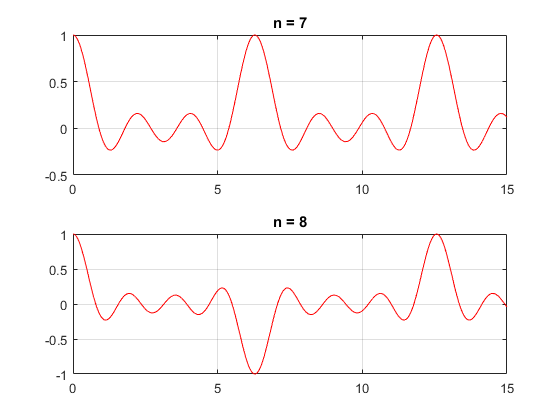
\includegraphics[width=\linewidth]{img_diric}
  \caption{Функция Дирихле нечетного (сверху) и четного (снизу) порядка.}
  \label{fig:img_diric}
\end{figure}

\subsubsection{Генерация сигнала с меняющейся частотой}
Функция \verb|y=chirp(t, f0, t1, fl, 'method', phi)| предназначена для генерации колебаний с единичной амплитудой, \emph{мгновенная частота} которых меняется по заданному закону. Здесь \verb|t| -- вектор значений времени, \verb|phi| -- начальная фаза колебания. Остальные параметры определяют закон изменения частоты.

Строковый параметр '\verb|method|' определяет тип зависимости мгновенной частоты от времени -- '\verb|linear|', '\verb|quadratic|' или '\verb|logarithmic|'. Метематически они описываются следующим образом:
\begin{description}
	\item['linear']:
	{
		\begin{equation}
		f(t)=f_0+ \beta t, \textrm{где $\beta=\frac{f_1-f_0}{t_1}$};
		\end{equation}
	}
	
	\item['quadratic']:
	{
		\begin{equation}
		f(t)=f_0+ \beta t^2, \textrm{где $\beta=\frac{f_1-f_0}{t_1^2}$};
		\end{equation}
	}
	
	\item['logarithmic']:
	{
		\begin{equation}
		f(t)=f_0+ e^{\beta t}, \textrm{где $\beta=\frac{ln(f_1-f_0)}{t_1}$};
		\end{equation}
	}
\end{description}

Ниже првиеден пример формирования трех сигналов, определенных на промежутке 0\ldots{}1 с и имеющих разные законы изменения мгновенной частоты.
\begin{verbatim}
Fs = 8e3;     % частота дискретизации
t = 0:1/Fs:1; % дискретное время
f0 = 1e3;
t1 = 1;
f1 = 2e3;
s1 = chirp(t,f0,t1,f1,'linear');
s2 = chirp(t,f0,t1,f1,'quadratic');
s3 = chirp(t,f0,t1,f1,'logarithmic');
specgram(s1,[],Fs)
title('linear');
colormap gray;
figure;
specgram(s2,[],Fs)
title('quadratic');
colormap gray;
figure;
specgram(s3,[],Fs)
title('logarithmic');
colormap gray;
\end{verbatim}

На Рис.~\ref{fig:img_chirp1}-\ref{fig:img_chirp3} изображены спектрограммы сформированных сигналов, наглядно демонстрирующие характер изменения мгновенной частоты при различных значениях параметра '\verb|method|'.
\begin{figure}[H]
  \centering
  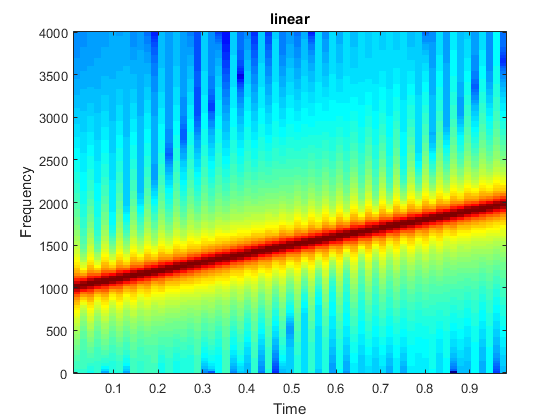
\includegraphics[scale=0.8]{img_chirp1}
  \caption{Спектрограмма сигнала, сформированного функцией chirp при линейном законе изменения мгновенной частоты.}
  \label{fig:img_chirp1}
\end{figure}
\begin{figure}[H]
  \centering
  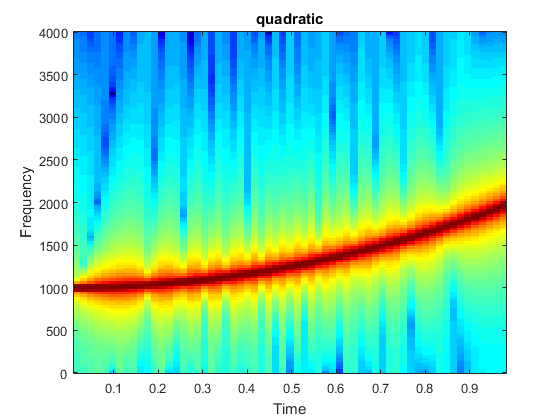
\includegraphics[scale=0.8]{img_chirp2}
  \caption{Спектрограмма сигнала, сформированного функцией chirp при квадратичном законе изменения мгновенной частоты.}
  \label{fig:img_chirp2}
\end{figure}
\begin{figure}[H]
  \centering
  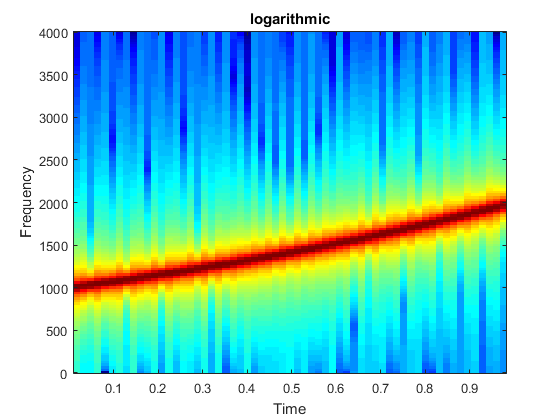
\includegraphics[scale=0.8]{img_chirp3}
  \caption{Спектрограмма сигнала, сформированного функцией chirp при экспоненциальном законе изменения мгновенной частоты.}
  \label{fig:img_chirp3}
\end{figure}
%\subsection{Теоретический раздел, содержащий основные соотношения между наблюдаемыми в работе явлениями}
%
%наблюдать поведение сигналов.

\subsection{Вывод}
Сигнал – физическая величина, изменяющаяся в зависимости от времени и/или пространственной переменной или набора (вектора) переменных (многомерные сигналы).

Классификация сигналов представляет собой две группы: \textbf{детерминированные} и \textbf{случайные}. В зависимости от того, известен ли сигнал \emph{точно}. 
В данной работе был рассмотрен класс детерминированных сигналов. Однако, возможность генерации случайных сигналов есть, проблема их генерации состоит в том, что они могут быть предсказаны лишь с некоторой вероятностью и отображают случайное физическое явление или физический процесс, причем зарегистрированный в единичном наблюдении сигнал не воспроизводится при повторных наблюдениях и не может быть описан явной математической зависимостью.

При анализе систем, в качестве тестовых сигналов используют детерменированные, так как в этом случае важно знать точный сигнал.

Если сигнал может быть описан функцией $s(t)=s(t+T)$, где $T$ -- период, он называется \textbf{периодическим}. Если сигнал невозможно описать функцией, он называется \textbf{непериодическим}.

По времени сигналы могут делиться на \textbf{непрерывные} и \textbf{дискретные}.

Существуют и другие критерии классификации сигналов. Например, различают ауди- и видеосигналы, с конечной и бесконечной энергией, широкополосные и узкополосные и так далее.

В пакете математического обеспечения MATLAB есть расширение Signal Processing,в котором имеются следующие функции, генерирующие часто встречающиеся на практике непериодические сигналы (одиночные импульсы):
\begin{description}
\item[rectpuls] -- прямоугольный импульс;
\item[tripuls] -- треугольный импульс;
\item[sinc] -- импульс вида $sin(\pi t)/(\pi t)$;
\item[gauspuls] -- радиоимпульс с гауссовской огибающей;
\item[pulstran] -- последовательность из конечного числа импульсов произвольной формы.
\end{description}

Кроме того, реализованы функции, позволяющие формировать отсчеты периодических сигналов различной формы:
\begin{description}
\item[square] -- последовательность прямоугольных импульсов;
\item[sawtooth] -- последовательность треугольных импульсов;
\item[diric] -- функция Дирихле.
\end{description}

\end{document}